\documentclass[notitlepage]{article}
\usepackage[T1, T2A]{fontenc}
\usepackage[utf8]{inputenc}
\usepackage[russian]{babel}
%
%\usepackage{newtxmath}
%\usepackage {fouriernc} %bold
%\usepackage{kpfonts}
%%
%\usepackage{gentium}
%\usepackage[default]{droidserif}
%\usepackage{XCharter} %bold
%
\usepackage{tikz, enumerate, graphicx, amsmath, amssymb, physics, caption}
\usepackage[section]{placeins}
\usepackage[separate-uncertainty=true, 
exponent-product={}\cdot, output-decimal-marker={,}]{siunitx}
\usetikzlibrary{calc,intersections, decorations.pathreplacing}
\newcommand{\intl}{\int\limits}
\newcommand{\intlinf}{\int\limits_{-\infty}^{+\infty}}
\newcommand\inner[2]{\left\langle #1, #2 \right\rangle}
\newcommand{\yav}[2]{\num{#1}\,\text{#2}}
\let\epsilon\varepsilon
\newcommand{\fpageplot}[4][90]
{\begin{figure}
  \caption{#4}
  \includegraphics[angle=#1, height=\textheight, width=\textwidth, keepaspectratio]
  {#2}
  \label{#3}
\end{figure}
}
\usepackage[a4paper, left=2cm, right=2cm, top=3cm, bottom=3cm]{geometry}
\title{Второе задание по методам оптимизации}
\author{Иван Ермаков}
\date{}
\begin{document}
\maketitle
\section*{3}
Логистическая регрессия
\begin{equation}
  \min_{x \in \mathbb{R}^n} \left\{f(x) = \frac 1m\inner{\ln\left[1 + \exp\left(-b \odot \left(A x\right)\right)\right]}{1_m}
  + \frac{\lambda}2 \norm{x}^2\right\}
\end{equation}
Здесь $b$ --- вектор из $b_i$, $A$ -- матрица $m \times n$, в которой строки являются векторами $a_i$.

\begin{equation}
  \begin{aligned}
    \operatorname{D} f(x) &= \lambda x - \frac {A^T} m\left(b\odot\frac{\exp\left(-b \odot \left(A x\right)\right)}
  {1 + \exp\left(-b \odot \left(A x\right)\right)}\right) = 
  \lambda x - \frac {A^T} m\left(b\odot u\left[-b\odot \left(A x\right)\right]\right)\\
  u(y) &= \frac{e^y}{1 + e^y} = \frac1{1 + e^{-y}}
  \end{aligned}
\end{equation}
Здесь использовано много свойств произведения Адамара.

\begin{equation}
    \dv{u}{y} = \frac{e^y(1 + e^y) - e^{2y}}{(1 + e^y)^2} = \frac{e^y}{(1 + e^y)^2}\\
    \end{equation}
\begin{equation}
  \operatorname{D}^2 f[\dd x] = \lambda \dd x + \frac {A^T}m \left(b\odot \frac{e^y}{(1 + e^y)^2} \odot b \odot \left(A \dd x \right)\right)
    \end{equation}
\begin{equation}
  \operatorname{D}^2 f = 
  \lambda + \frac {A^T}m \left\{\left[\left(b \odot b \odot \frac{e^y}{(1 + e^y)^2}[-b \odot (Ax)]\right) 1_n^T\right] \odot A\right\}
\end{equation}
Потратив еще \textit{немного} времени, можно понять, что это выражение можно переписать как
\begin{equation}
  \operatorname{D}^2 f = \lambda + \frac 1m \cdot A^T \operatorname{diag}\left\{b\odot b \odot v(-b \odot \left(A x\right))\right\} A
\end{equation}
где
\begin{equation}
  v(y) = \frac{e^y}{(1 + e^y)^2}
\end{equation}
\section{Эксперимент: траектория градиентного спуска}
Построение графиков выполнено при помощи скрипта ``grad\_trajectory.py''. 
\begin{figure}[ht]
\begin{minipage}[t]{.5\textwidth}
  \centering
  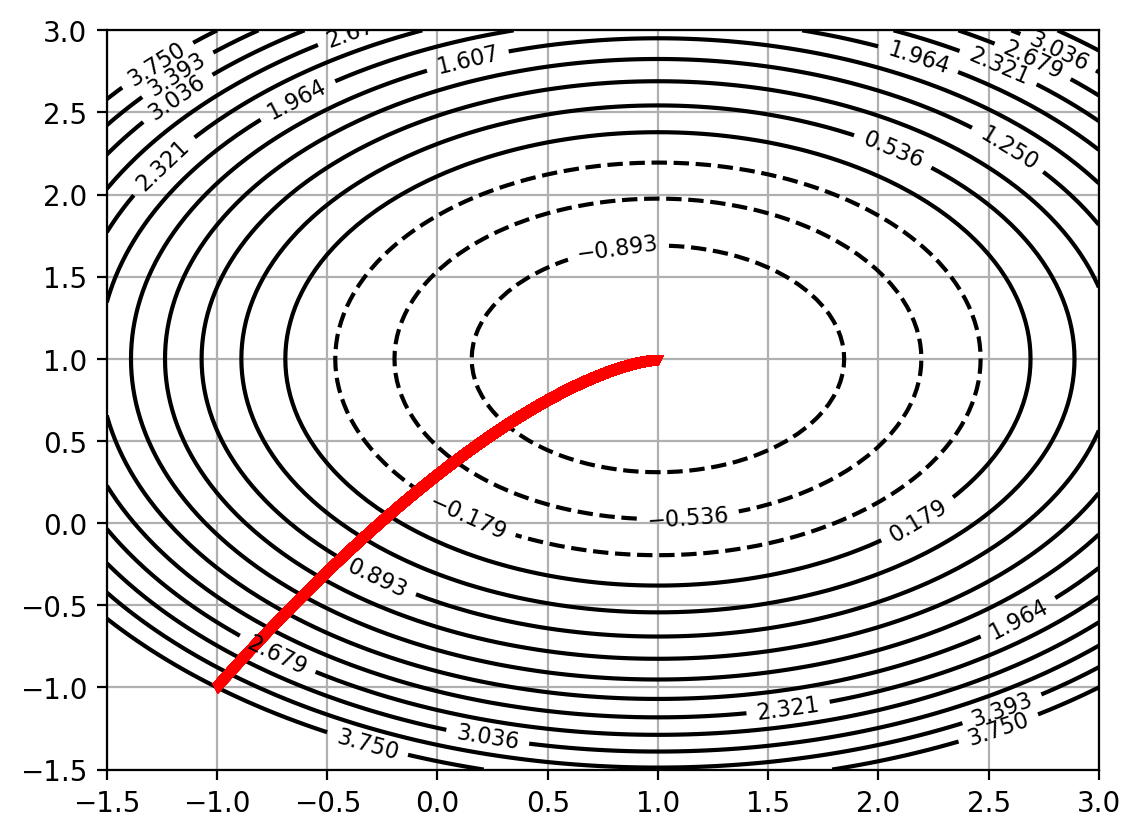
\includegraphics[width=\textwidth, keepaspectratio]{plots/trajectory_0_0.png}
  \captionof{figure}{Постоянный шаг, хорошо обусловленная матрица.}
\end{minipage}
\begin{minipage}[t]{.5\textwidth}
  \centering
  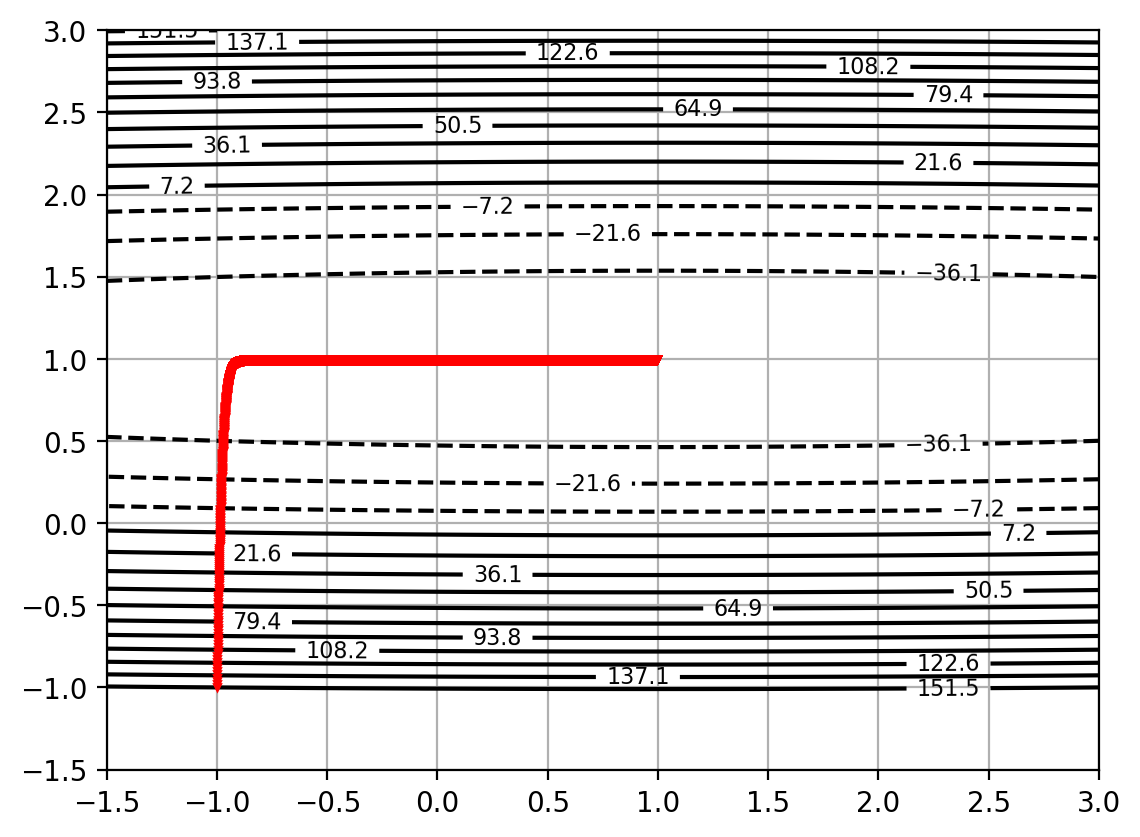
\includegraphics[width=\textwidth, keepaspectratio]{plots/trajectory_1_0.png}
  \captionof{figure}{Постоянный шаг, плохо обусловленная матрица.}
\end{minipage}
\end{figure}
Для хорошо обусловленной матрицы поиск останавливается за 109000 шагов, а для плохо обусловленной за 69000.
Скорее всего так происходит из-за того, что в хорошо обсусловленной матрице метод постоянно проскакивает оптимальную точку
из-за высокой требуемой точности.

\begin{figure}[ht]
\begin{minipage}[t]{.5\textwidth}
  \centering
  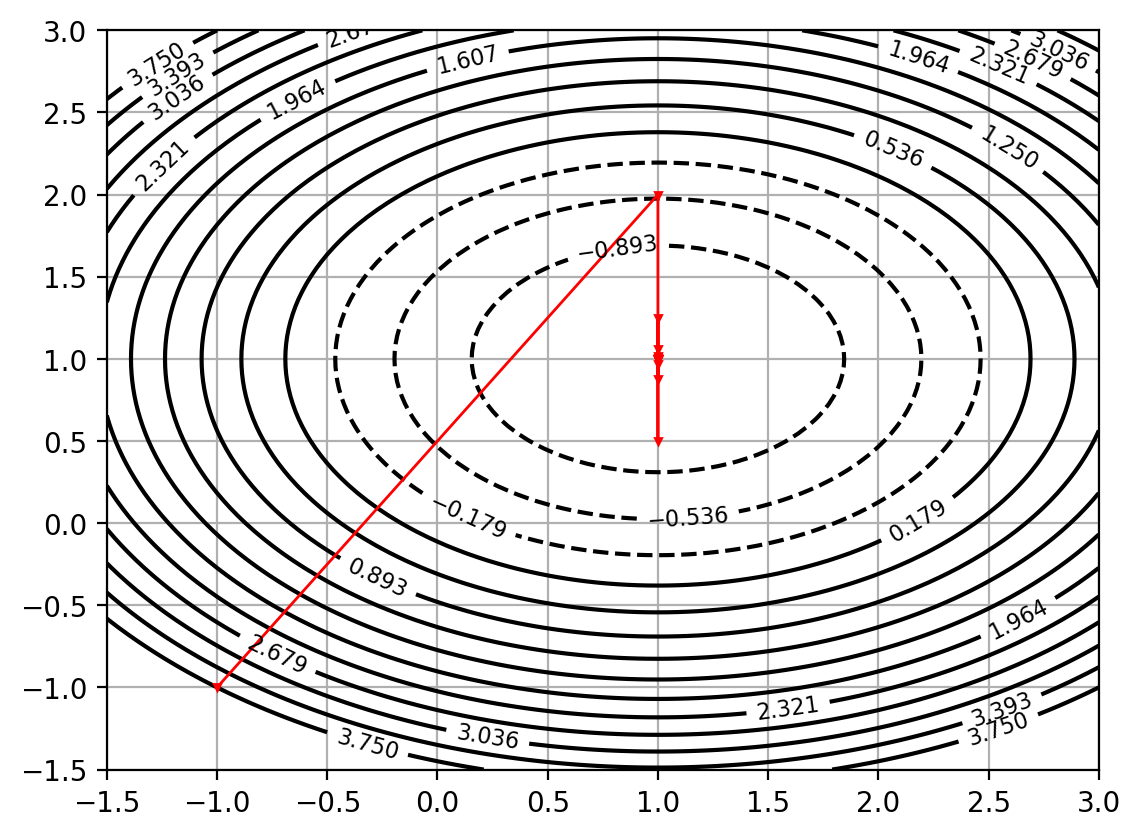
\includegraphics[width=\textwidth, keepaspectratio]{plots/trajectory_0_1.png}
  \captionof{figure}{Условие Армихо, хорошо обусловленная матрица.}
\end{minipage}
\begin{minipage}[t]{.5\textwidth}
  \centering
  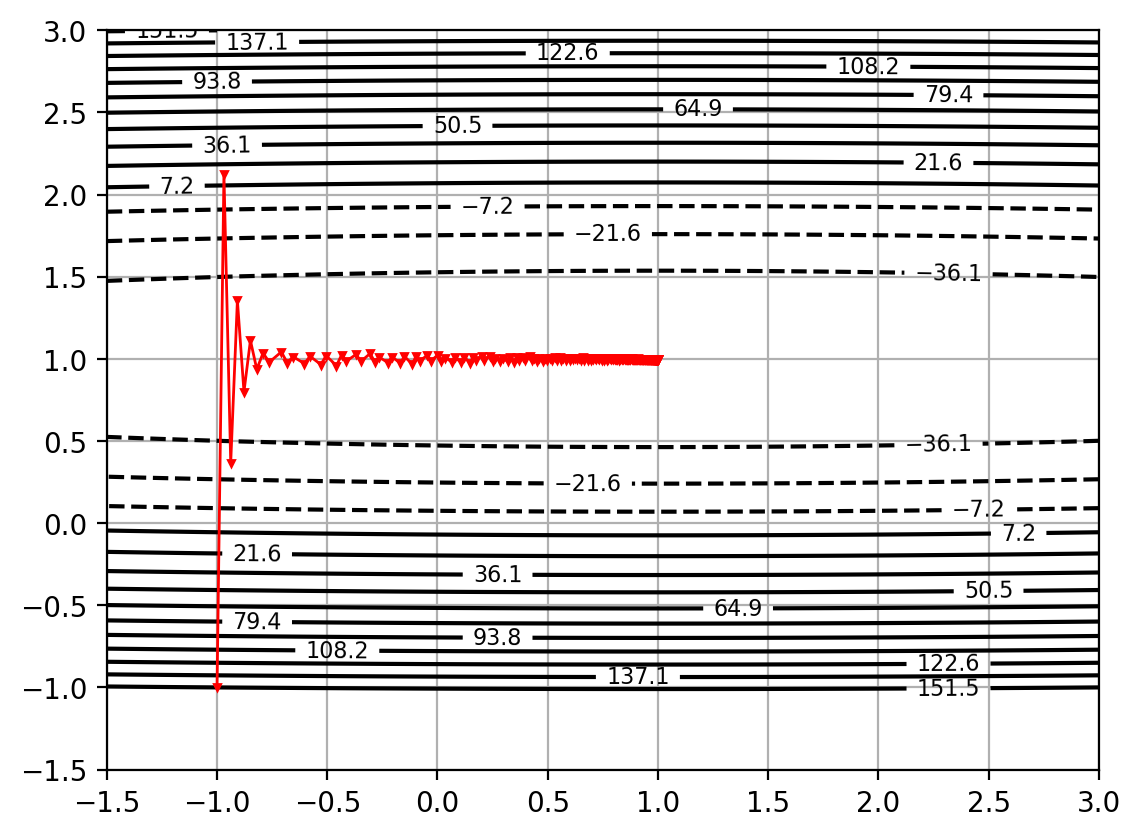
\includegraphics[width=\textwidth, keepaspectratio]{plots/trajectory_1_1.png}
  \captionof{figure}{Условие Армихо, плохо обусловленная матрица.}
\end{minipage}
\end{figure}
Теперь все встало на свои места: для хорошо обусловленной матрицы метод сходится всего за 18 шагов. Для плохо обусловленной
требуется 327 шагов. Видно, что в первом случае довольно быстро тракетория становится прямой, а во втором случае она все время
колеблется вокруг оптимального пути и совершает больше шагов, чем нужно.

\begin{figure}[ht]
\begin{minipage}[t]{.5\textwidth}
  \centering
  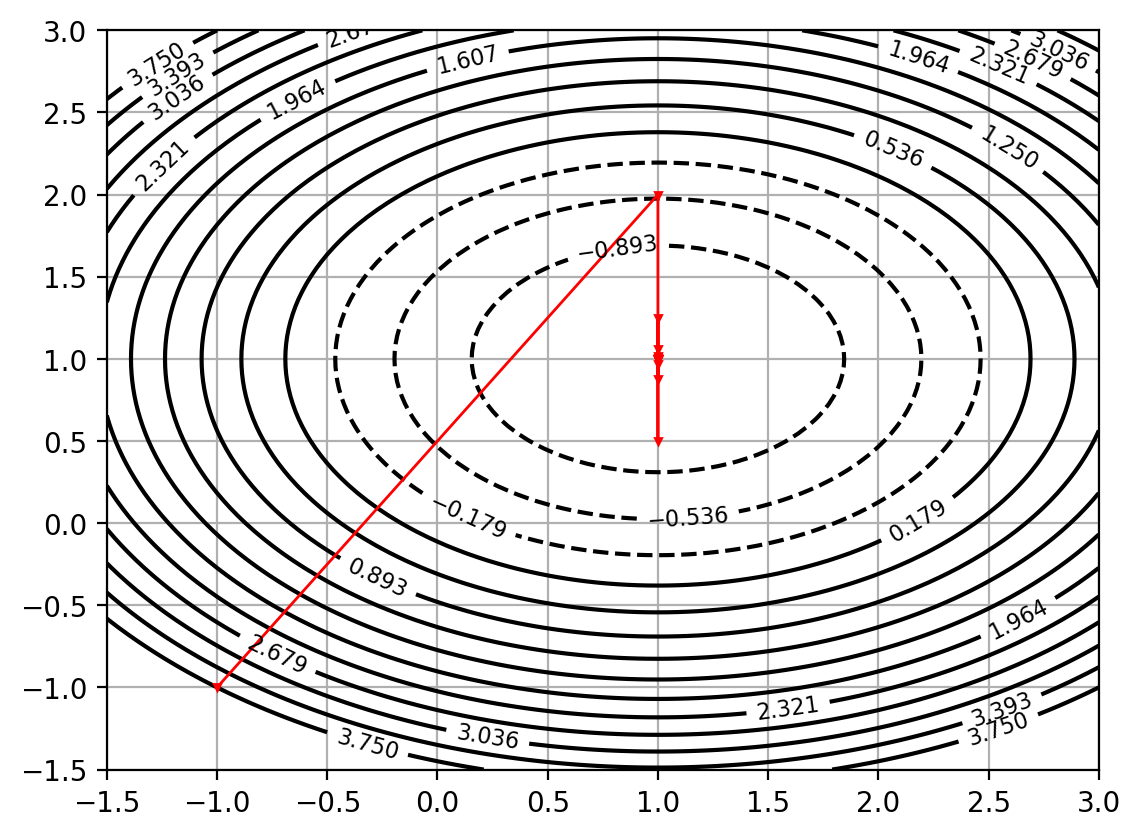
\includegraphics[width=\textwidth, keepaspectratio]{plots/trajectory_0_2.png}
  \captionof{figure}{Условие Вольфа, хорошо обусловленная матрица.}
\end{minipage}
\begin{minipage}[t]{.5\textwidth}
  \centering
  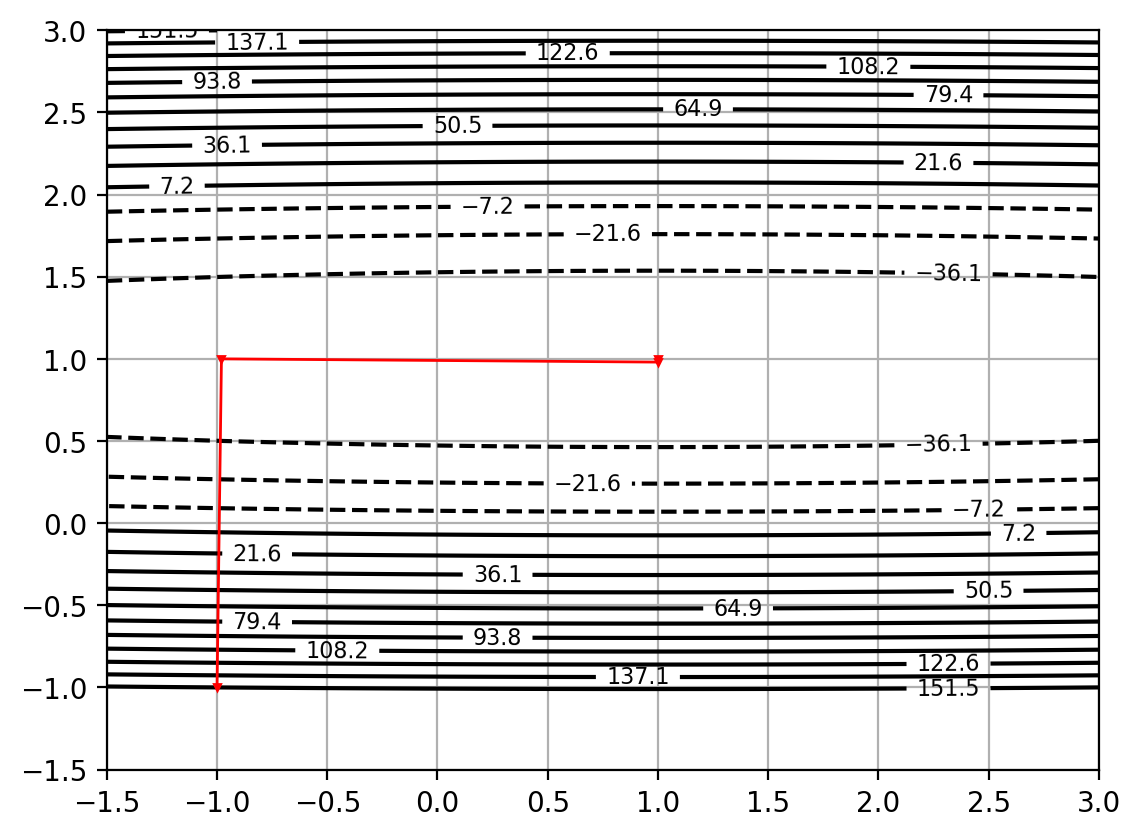
\includegraphics[width=\textwidth, keepaspectratio]{plots/trajectory_1_2.png}
  \captionof{figure}{Условие Вольфа, плохо обусловленная матрица.}
\end{minipage}
\end{figure}
Для условия Вольфа ситуация аналогичная первому случаю: для хорошо обусловленной матрицы метод работает ``слишком хорошо'' и
проскакивает точку экстремума. Метод сходится за 18 шагов. Для плохо обусловленной матрицы требуется всего 4 шага.
Понятно, что в общем случае для хорошо обусловленой матрицы метод Вольфа тоже работает хорошо, и некоторое $O(1)$ количество
операций в конце, связанное с проскакиванием, роли не играет.

При этом, конечно, чем ближе прямая градиента к оптимальной точке, тем быстрее будут работать все методы, потому что траектория будет
ближе к прямой.

\section*{Эксперимент: зависимость числа итераций итераций градиентного спуска от числа обусловленности и размерности пространства}
Выборка генерируется при помощи скрипта ``perf\_plots.py'' так, как ьыло рекомендовано в задании:
генерируется диагональная матрица, далее у нее фиксируется число обусловленности. Потом случайным образом выбираются $x_0$ и $b$.
Получившиеся семейства кривых изображены на рисунке \ref{fig:perfplot}
\begin{figure}[ht]
  \centering
  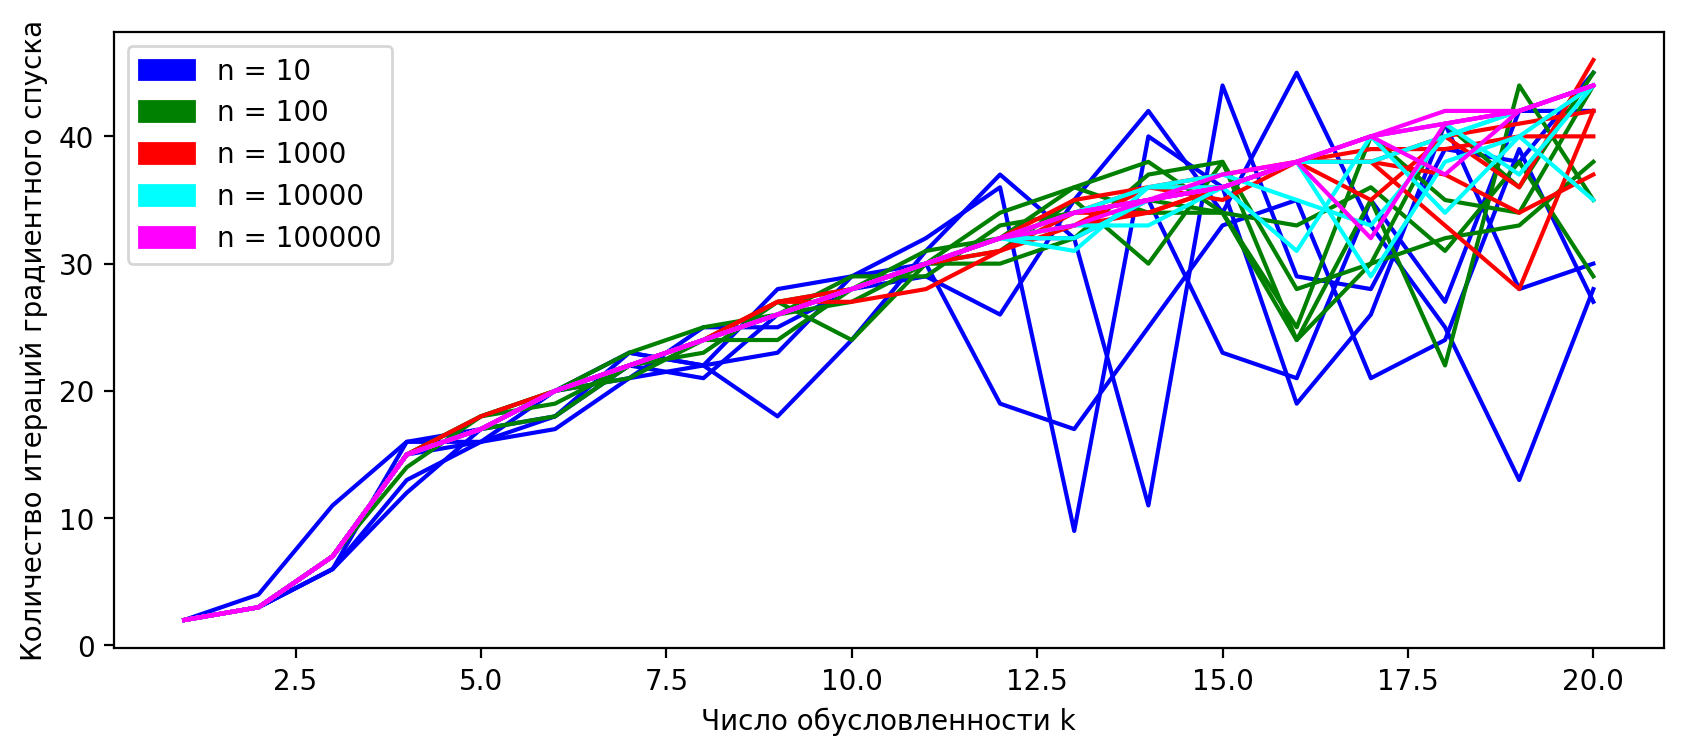
\includegraphics[width=\linewidth, keepaspectratio]{plots/perf_gradients.png}
  \caption{Зависимость числа итераций от числа обусловленности и размерности пространства}
  \label{fig:perfplot}
\end{figure}

Видно, что от размерности пространства количество итераций не зависит. А вот с ростом числа обусловленности количество
итераций растет. Причем рост, хотя это и сложно определить, похож на линейный. Линейный рост можно объяснить так:
\begin{equation}
  f(x_k) - f^* \leq \frac L2 \left(\frac{\kappa - 1}{\kappa + 1}\right)^{2k} \norm{x_0 - x^*}^2
\end{equation}
Отсюда
\begin{equation}
  k = \frac{\ln\alpha}{2\ln\left(\dfrac{\kappa - 1}{\kappa + 1}\right)} \approx -\kappa\ln\alpha 
\end{equation}
из Тейлоровского разложение при $\kappa \gg 1$.

\section*{Эксперимент: Сравнение методов градиентного спуска и Ньютона на реальной задаче логистической регрессии}

На одну итерацию градиентному спуску требуется $O(n)$ памяти, поскольку хранятся только векторы $x$ и $\nabla f$. 
Матрица, конечно, тоже хранится, но она разреженная и не занимает много памяти.
Подсчет градиента требует $O(nm)$ времени для умножения матрицы на вектор.
Линейный поиск также требует $O(nm)$ операций, поскольку для вычисления значения функции тоже нужно умножать матрицу.
Для сложения координат нужно $O(n)$ операций. В итоге требуется $O(nm)$ времени для одного шага градиентного спуска.

Метод Ньютона требует $O(n^2)$ памяти на каждом шаге, поскольку разложение Холецкого из scipy не поддерживает разреженные
матрицы, и внутри неявным образом она приводится к обычной плотной матрице.
Для обращения гессиана(или, эквивалентно, для решения СЛАУ) требуется $O(n^3)$ операций.
Для последующего линейного поиска требуется $O(nm)$ операций. В итоге получается сложность операции $O(nm + n^3)$.

У меня получилось выполнить на своем компьютере с $16$\,Гб оперативной памяти все вычисления, кроме метода Ньютона для
датасета real-sim.
Матрица из этого датасета, если хранить ее как плотную матрицу,
при представлении в виде плавающих чисел с одинарной точностью занимает в памяти $5.6$\,Гб.
Разреженная матрица занимает в памяти намного меньше места.
Однако, как было отмечено выше, разложение Холецкого неявно превращает матрицу в плотную.
Более того, видимо, из-за особенностей аллокации numpy, на второй итерации метода количество памяти еще возрастает.
Поэтому тесты для этого датасета были выполнены на кластере ЦОД МФТИ используя $32$\,Гб оперативной памяти.
Для возможности сравнивать время обработки разных датасетов все вычисления в итоге были выполнены на кластере.

\begin{figure}[ht]
\begin{minipage}[t]{.5\textwidth}
  \centering
  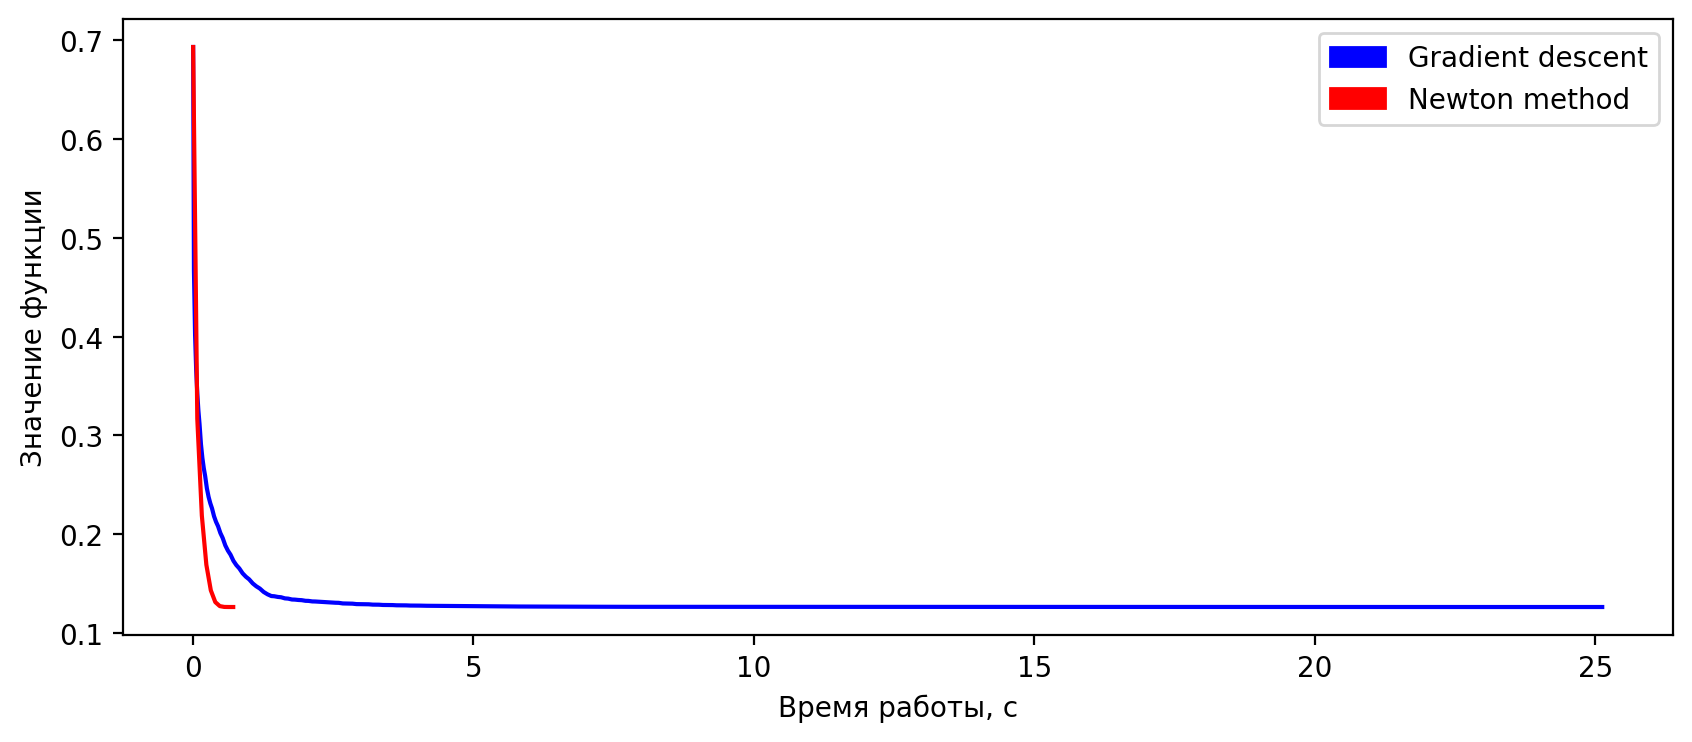
\includegraphics[width=\textwidth, keepaspectratio]{plots/w8a_plot_func.png}
  \captionof{figure}{Датасет w8a, значения функции}
\end{minipage}
\begin{minipage}[t]{.5\textwidth}
  \centering
  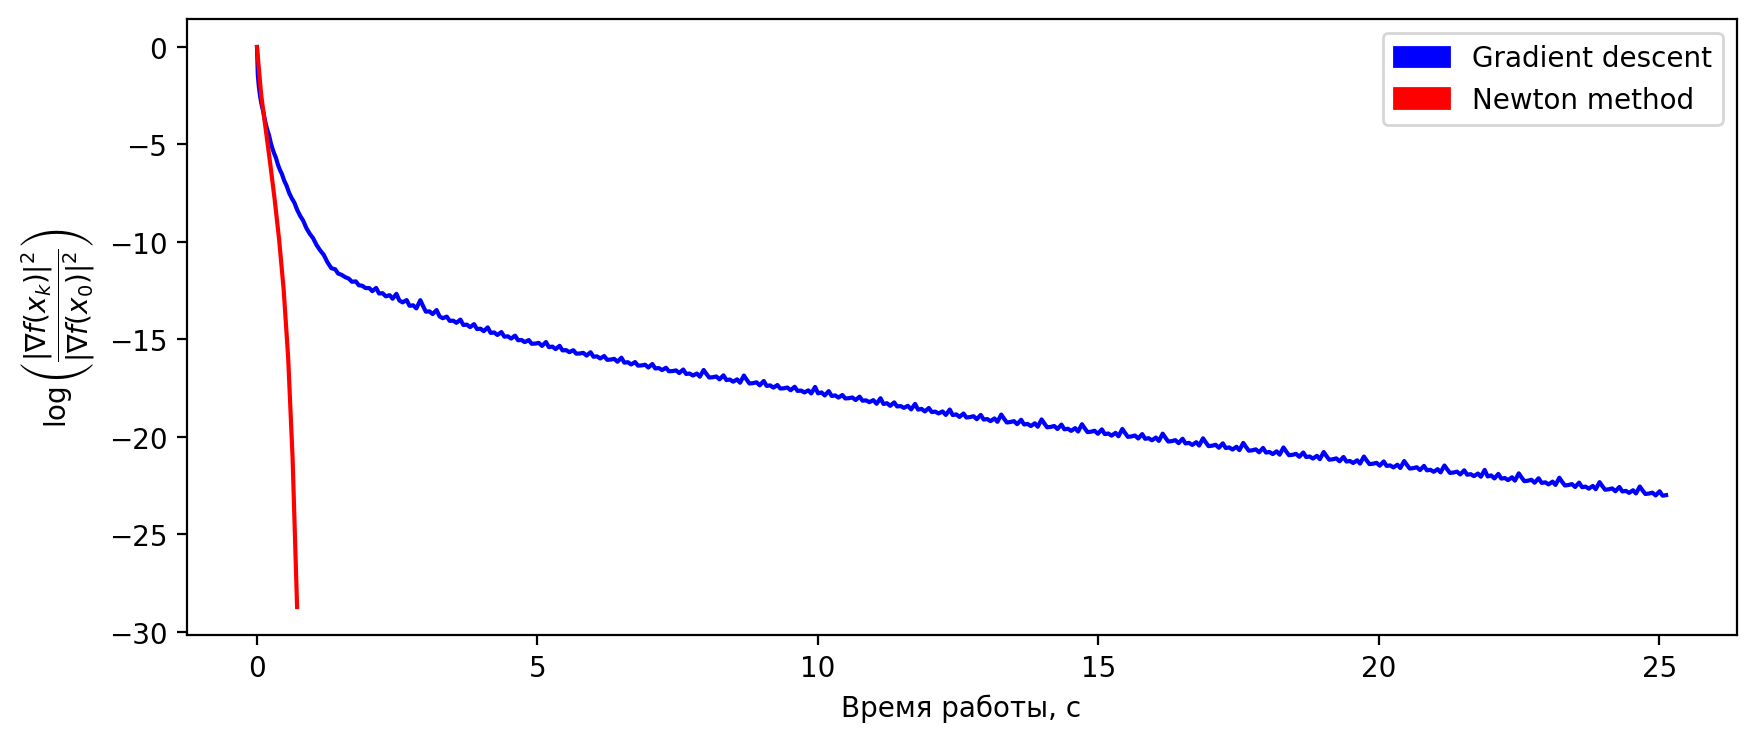
\includegraphics[width=\textwidth, keepaspectratio]{plots/w8a_plot_grad.png}
  \captionof{figure}{Датасет w8a, значения градиента}
\end{minipage}
\end{figure}
\begin{figure}[ht]
\begin{minipage}[t]{.5\textwidth}
  \centering
  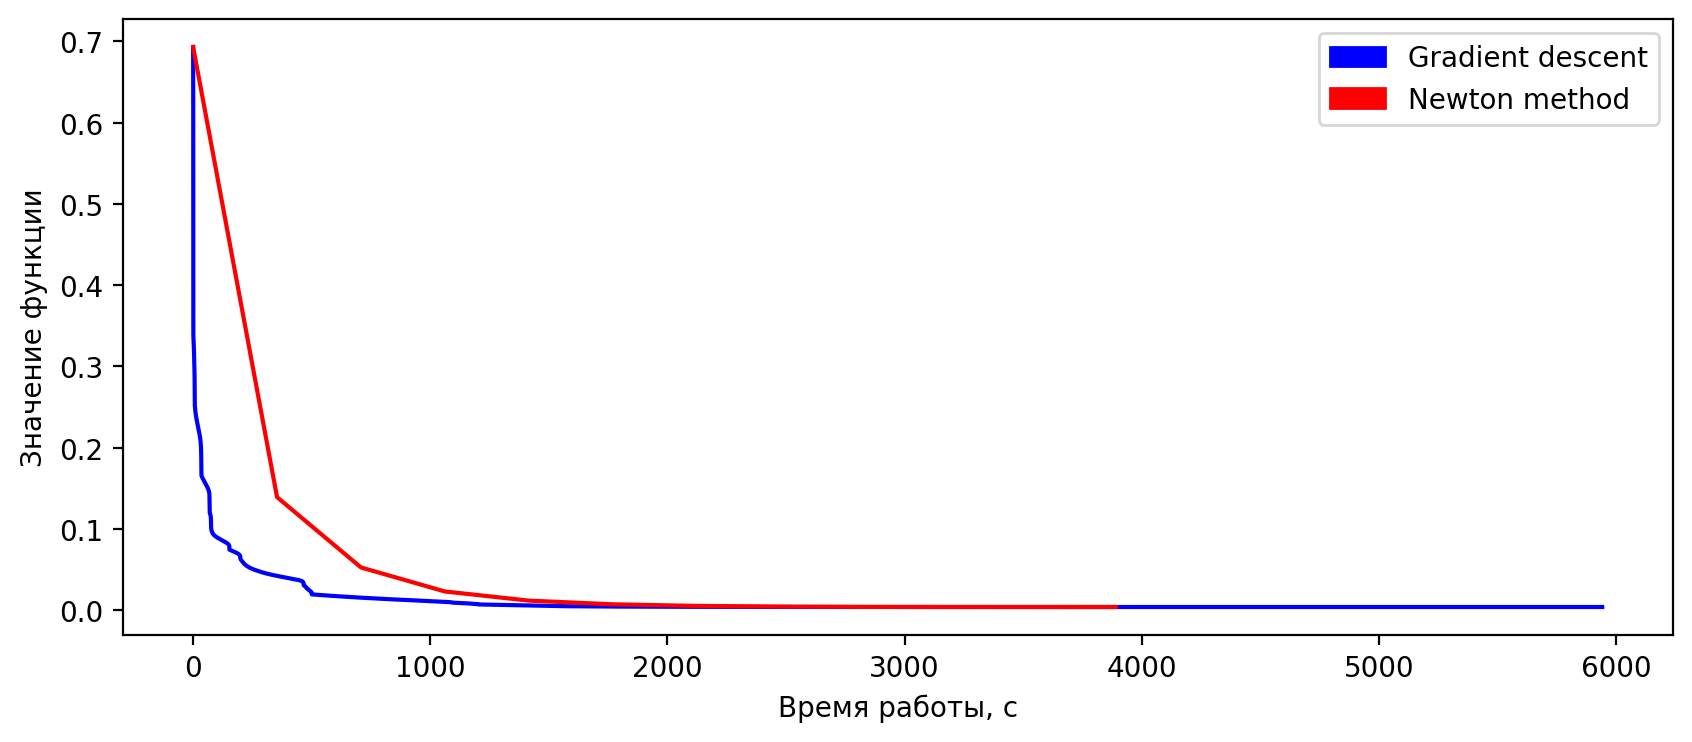
\includegraphics[width=\textwidth, keepaspectratio]{plots/gisette_scale.bz2_plot_func.png}
  \captionof{figure}{Датасет gisette, значения функции}
\end{minipage}
\begin{minipage}[t]{.5\textwidth}
  \centering
  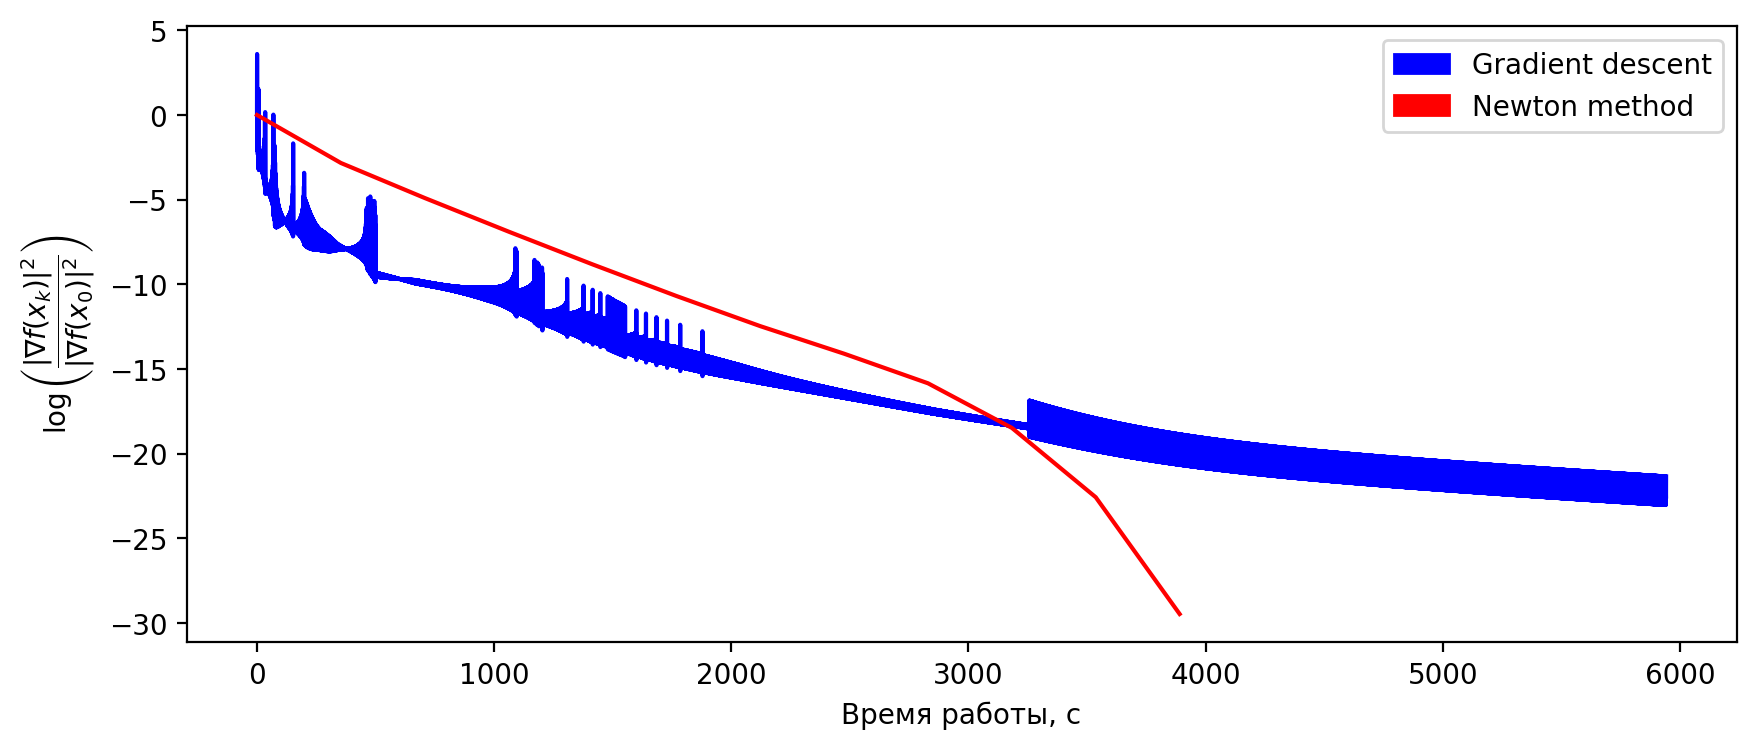
\includegraphics[width=\textwidth, keepaspectratio]{plots/gisette_scale.bz2_plot_grad.png}
  \captionof{figure}{Датасет gisette, значения градиента}
\end{minipage}
\end{figure}
\begin{figure}[ht]
\begin{minipage}[t]{.5\textwidth}
  \centering
  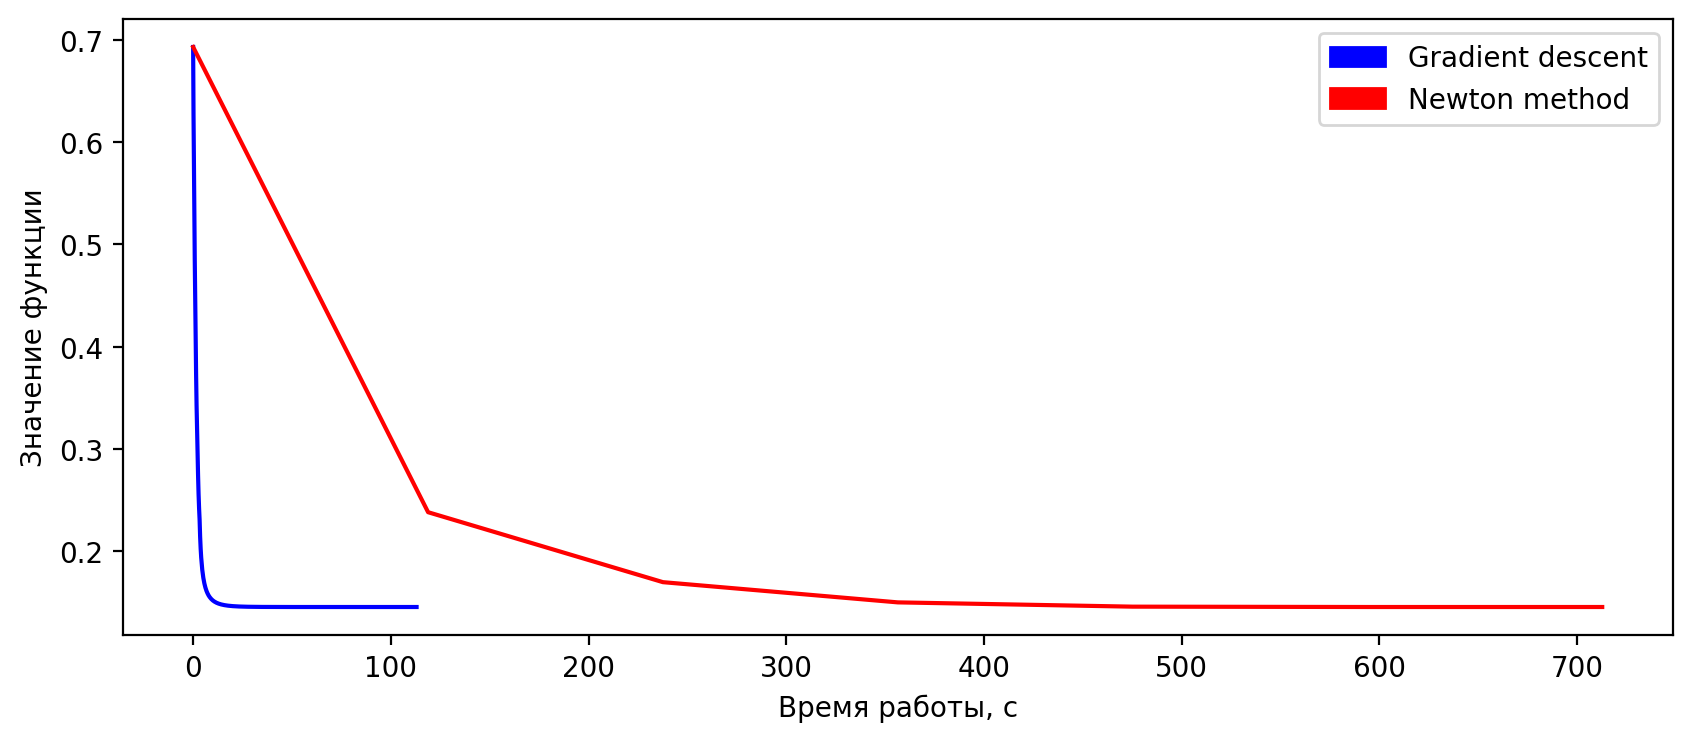
\includegraphics[width=\textwidth, keepaspectratio]{plots/real-sim.bz2_plot_func.png}
  \captionof{figure}{Датасет real-sim, значения функции}
\end{minipage}
\begin{minipage}[t]{.5\textwidth}
  \centering
  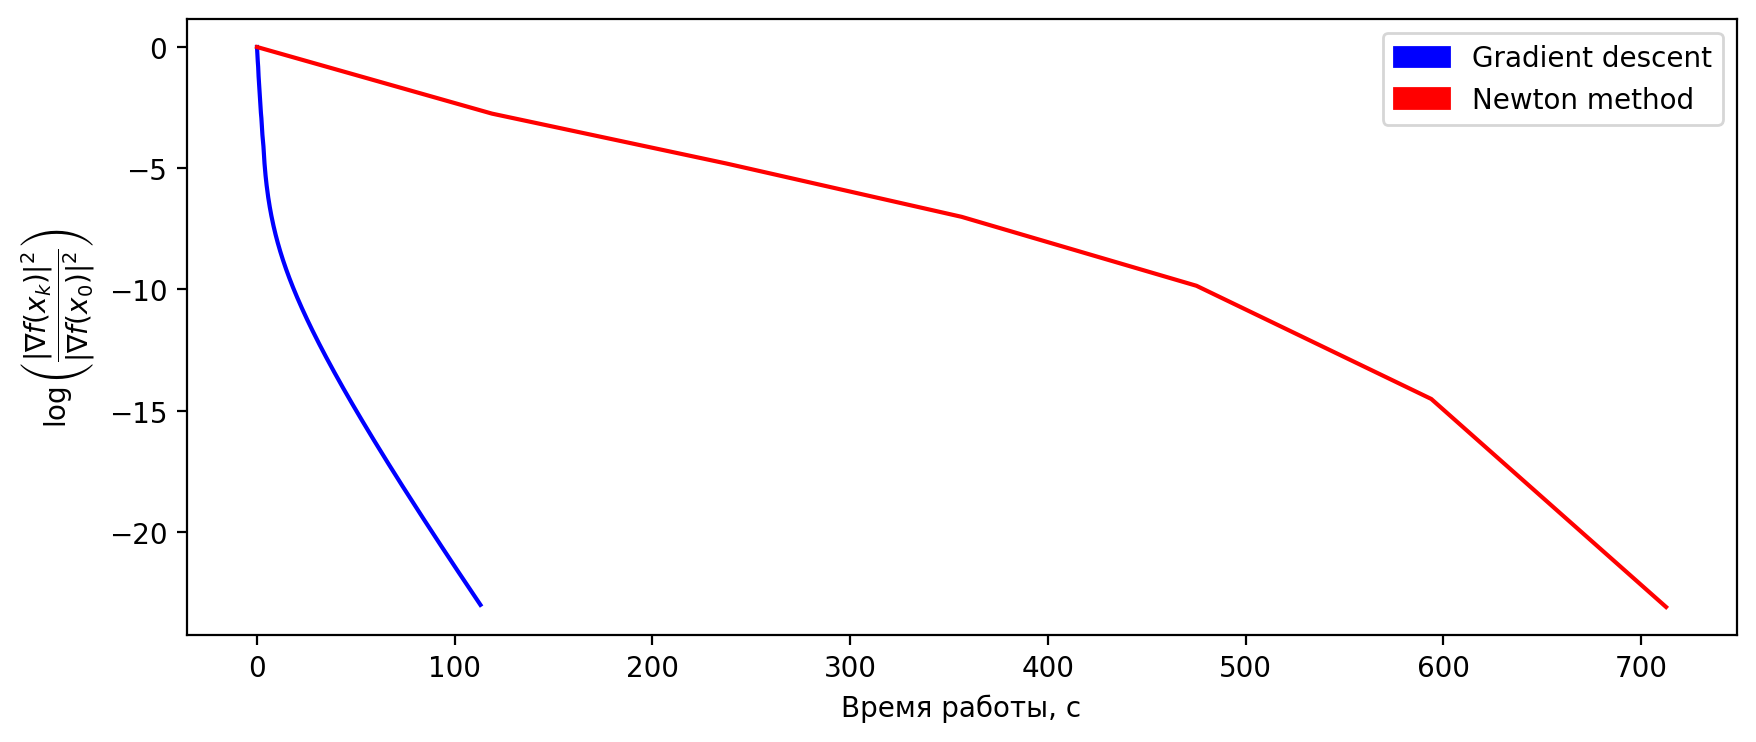
\includegraphics[width=\textwidth, keepaspectratio]{plots/real-sim.bz2_plot_grad.png}
  \captionof{figure}{Датасет real-sim, значения градиента}
\end{minipage}
\end{figure}

\large\textbf{Выводы:}
Если посмотреть на графики, становится видно, что метод Ньютона для большинства датасетов работает быстрее из-за сверхлинейной
скорости сходимости.
Однако для больших $n$, когда $n^3$ становится очень уж большим, градиентный спуск начинает выигрывать, поскольку
количество итераций градиентного спуска и метода Ньютона не зависят от размерностей.

Также интересно отметить колебания градиента функции в градиентном спуске.
Это, по видимости, связано с тем, что линейный поиск выбирает
достаточно большую длину шага для того, чтобы на ней градиент заметно изменился.
Можно предположить, что происходят осцилляции в направлениях, заметно отличающихся от направления к минимуму, то есть задача в данных точках плохо обусловлена.

Градиентный спуск лучше для очень большого количества признаков, то есть для большого числа $n$.
При этом желательно, чтобы в данных не было выбросов, так как это потенциально может привести к плохой обусловленности задачи.
Метод Ньютона хорош для достижения высокой точности из-за сверхлинейной скорости сходимости, однако он требует 
большого количества памяти и не подходит для очень больших $n$.

Хочется попробовать использовать scikit-sparse, который поддерживает разложение Холецкого для разреженных матриц.
По игоам экспериментов оказалось, что использование этого пакета действительно сильно снижает использование памяти.
Все тесты стало возможно выполнить на 16\,Гб оперативной памяти.
Код, использующий scikit-sparse расположен в другой ветке репозитория, поэтому в прилагаемые файлы не вошел.

			
			
\end{document}
